%!TEX root = ../proposal.tex
\section{Proposed Method}\label{sec:proposedMethod}
The following section explains all proposed strategies and solutions implemented by \drivebuild{} for formalizing test cases and for specifying the life cycle handling the execution of tests.\\
Therefore this section describes the scheme for the test case formalization, the life cycle of tests, the runtime verification of criteria and the proposed cluster architecture.

\subsection{Test Case Formalization}
\begin{table}
    \centering
    \caption{%
        Target \glspl{adas} --- This table lists all \glspl{adas} that the formalization aims to support.
        The \glspl{adas} are grouped based on their functionality and thus by the data they require to work.
    }
    \medskip
    \def\tabularxcolumn#1{m{#1}}
    \begin{tabularx}{\linewidth}{c l X}
        \toprule
        \bfseries Group & \bfseries To be supported & \bfseries Description \\
        \midrule
        1 & \mltc[@{}l]{%
            Collision avoidance system\\
            Forward Collision Warning\\
            Emergency Brake Assist\\
            Intersection assistant\\
            Turning assistant
        } & Systems that alert a driver with a warning, avoid or reduce the severity of a collision and actively brake an \gls{av}\\
        \midrule
        2 & \mltc[@{}l]{%
            Cruise control\\
            Intelligent speed adaptation\\
            Adaptive cruise control\\
            Active Brake Assist
        } & Systems that control the speed of an \gls{av} making sure it does not exceed a certain speed limit or maintains a safe distance to other participants\\
        \midrule
        3 & \mltc[@{}l]{%
            Lane centering\\
            Lane departure warning system\\
            Lane change assistance\\
            Wrong-way driving warning
        } & Systems that observe the relative position of an \gls{av} on the road and that make sure it does not leave the lane it is supposed to drive on\\
        \midrule
        4 & Adaptive light control & A system that controls the lights depending on the brightness and whether another participant comes towards\\
        \bottomrule
    \end{tabularx}\label{table:targetAdas}
\end{table}
There is no standard specifying reference test cases and their expected results~\cite{noStandard}.
Since \glspl{adas} are safety critical the formalization in this work concentrates on \glspl{adas} that can be tested using simulations.
\autoref{table:targetAdas} lists the target \glspl{adas} and groups them by their functionality and the data these need to work.
\begin{table}
    \centering
    \caption{Minimum test data requirement --- This table lists the minimum required data for the groups of \glspl{adas} described in \autoref{table:targetAdas} to test them.}
    \medskip
    \def\tabularxcolumn#1{m{#1}}
    \begin{tabularx}{\linewidth}{X c c c c}
        \toprule
        \bfseries Type of data & \bfseries Group 1 & \bfseries Group 2 & \bfseries Group 3 & \bfseries Group 4 \\
        \midrule
        Distance to other traffic participants & \checkmark{} & \checkmark{} & \ding{53} & \checkmark{} \\
        Distance to lane markings and to the edges of the roads & \ding{53} & \checkmark{} & \checkmark{} & \ding{53}\\
        Relative speed to other traffic participants & \checkmark{} & \checkmark{} & \checkmark{} & \checkmark{}\\
        Damage detection & \checkmark{} & \checkmark{} & \ding{53} & \ding{53}\\
        Speed & \checkmark{} & \checkmark{} & \ding{53} & \ding{53}\\
        \bottomrule
    \end{tabularx}\label{tab:reqData}
\end{table}
The data \glspl{adas} require is heavily dependant on their implementation
Nevertheless based on their functionality there is a common basis of information required to test them (See \autoref{tab:reqData}).\\
The formalization follows a modular approach separating the description of environments on the one hand from the descriptions of participants and criteria on the other hand.
This allows to reuse environments throughout multiple scenarios and avoids duplication
\subsubsection{Formalization of Environments}
The definition of test environments follows a custom scheme since other currently well known schemes are not suitable as explained in \autoref{sec:problem}.
The scheme describes lanes and obstacles.
A lane is a sequence of tuples.
Each tuple contains the lane center point and the current width of the lane.
Since this representation is identical to the representation used by the simulator which I will use in my work and which is described in the proposed tools paragraph in \autoref{sec:testCycle} the expected outcome of the generated lanes is very similar to the test case definition.
Additionally this representation allows to easily calculate the distance of an \gls{av} to the lane center and to determine the direction of a lane.
An obstacle may be either a cube (having a position, width, length, height and rotation) or a cylinder/cone (having a position, radius, height and rotation).
\autoref{fig:exampleEnvironment} shows an example description and \autoref{fig:exampleEnvironmentVis} its visualization.
\begin{figure}
    \caption{Example environment description --- This example shows example definitions of a single slightly curvy lane and of the available shapes of static obstacles.}\label{fig:exampleEnvironment}
    \medskip
    \lstinputlisting[language=xml]{code/exampleEnvironment.dbe.xml}
\end{figure}
\begin{figure}
    \caption{Visualization of example environment --- This picture shows the generated environment described by \autoref{fig:exampleEnvironment}.}\label{fig:exampleEnvironmentVis}
    \medskip
    \includegraphics[width=\linewidth]{pictures/2019-06-04_simpleLaneWithObstacles.png}
\end{figure}
\subsubsection{Formalization of Participants}
Traffic participants are specified by an initial state, their movement and optionally by the data \glspl{ai} controlling them may require.
This includes especially the sensor data.
The shape and the physics of participants are specified by using a predefined model provided by the underlying simulator.
An initial state sets the initial position, the initial orientation and the initial movement mode, which is one of \ilmanual{}, \ilautonomous{} or \iltraining{}, of an \gls{av}.
A movement is a sequence of states.
Each state defines a target waypoint, optionally a speed value and a movement mode.
A waypoint is a position bundled with a tolerance value which allows a participant to not precisely reach a position but to pass by in a certain distance.
A speed value is either a target speed the \gls{av} should have or a speed limit the \gls{av} shall not exceed.
If the current movement mode of an \gls{av} is \ilmanual{} the car heads straight to the waypoint of the next state.
If the movement mode is \ilautonomous{} the \gls{ai} that registered for controlling the \gls{av} is frequently requested like explained in \autoref{sec:testCycle} and provided with data it needs to control the \gls{av}.
\begin{table}
    \caption{Available simulation data --- This table lists all types of data an \gls{ai} that registered at a simulation can possibly request and whether it can be considered as sensor data.}\label{tab:aiData}
    \medskip
    \begin{tabularx}{\linewidth}{l X c}
        \toprule
        \bfseries Type & \bfseries Description & \bfseries Sensor Data\\
        \midrule
        position & The absolute position of an \gls{av} & \ding{53}\\
        lane & The name of the lane an \gls{av} is currently on & \ding{53}\\
        distance to lane center & The distance to the center of the nearest lane & \checkmark{}\\
        speed & The absolute speed of an \gls{av} & \checkmark{}\\
        steering angle & The current steering angle of the steering wheel & \checkmark{}\\
        car to lane angle & The angle between the orientation of a participant and the center of the nearest lane & \ding{53}\\
        \glstext{lidar} & Data provided by a \gls{lidar} sensor & \checkmark{}\\
        camera & Camera images either colored, annotated or with depth information & \checkmark{}\\
        damage & Detects whether an \gls{av} is damaged & \checkmark{}\\
        light & Determines which lights are turned on & \checkmark{}\\
        \bottomrule
    \end{tabularx}
\end{table}
\autoref{tab:aiData} lists the types of data that an \gls{ai} can request and whether the data is considered as sensor data.
For having realistic \glspl{ai} only sensor data should be used for the \gls{ai} itself.
The other types of data can be used for collecting training data or for introducing additional criteria checked before or after the computations of an \gls{ai} like explained in \autoref{subsubsec:criteria}.
If the movement mode is set to \iltraining{} the \gls{av} acts the same way it does in \ilmanual{} but requests the \gls{ai} like in \ilautonomous{}.
In contrast to \ilautonomous{} the \gls{ai} can not control the \gls{av}.
However, the \gls{ai} can still control the simulation.
This mode is meant to be used for collecting training data for \glspl{ai}.
This scheme for movements enables to mix sections where an \gls{av} is forced to follow a path, where an \gls{ai} has to control it or where data has to be collected.
\autoref{fig:exampleParticipant} shows an example definition of a participant and \autoref{fig:exampleParticipant} show the corresponding graphical representation.
Additionally \autoref{sec:runtimeVerification} explains how \glspl{ai} communicate with a simulation.
\begin{figure}
    \caption{Example participant description --- This example shows an example of positioning a participant, defining its movement and which data its \gls{ai} requires.}\label{fig:exampleParticipant}
    \medskip
    \lstinputlisting[language=xml]{code/exampleMovement.dbc.xml}
\end{figure}
\begin{figure}
    \caption{%
        Visualization of example participant --- This picture shows the generated participant and its movement based on the description in \autoref{fig:exampleParticipant}.
        The image also visualizes also where the \gls{av} is in which movement mode.
        Green lines mark movements in the \ilmanual{} mode and the red section marks  a movement in the \ilautonomous{} mode.
    }\label{fig:exampleParticipantVis}
    \medskip
    \includegraphics[width=\linewidth]{pictures/2019-06-05_ParticipantMovement.png}
\end{figure}
\subsubsection{Formalization of Criteria}\label{subsubsec:criteria}
The test criteria definition specifies preconditions, success and fail criteria.
Commonly a test is considered as successful if it ends without triggering a fail criterion.
In the context of testing \glspl{av} a possible test might be ``An \gls{av} \(A\) is successful if it reaches a certain position \(P\) and fails if it takes any damage''.
Such test cases require to separate success from fail criteria since if \(A\) just does not move it does not fail but it is not successful either.
The most basic way of describing this is the Kleene and Priest logics~\cite{kleeneLogics} which is a three-valued logics declaring besides \iltrue{} and \ilfalse{} also \ilunknown{}.
This third value \ilunknown{} allows to express that a criterion could not be determined or is currently not considered.
The test criteria divide into connectives (\iland{}, \ilor{} and \ilnot{}), \glspl{sc} and \glspl{vc} and can be nested as shown in \autoref{fig:nesting}..
\begin{figure}
    \centering
    \caption{Nesting of criteria --- This diagram shows the allowed nesting structure for test criteria. Italic types are abstract.}\label{fig:nesting}
    \medskip
    \begin{tikzpicture}[%
            ->,
            >=stealth
        ]
        \node (evaluation) {\itshape evaluation};
        \node[above=of evaluation] (start) {};
        \node[below=of evaluation] (criterion) {\itshape criterion};
        \node[left=of criterion] (connective) {\itshape connective};
        \node[below=of connective] (and) {and};
        \node[right=of and] (or) {or};
        \node[left=of and] (not) {not};
        \node[below=of criterion] (sc) {\glstext{sc}};
        \node[right=of sc] (vc) {\glstext{vc}};

        \path
            (start) edge (evaluation)
            (evaluation) edge (criterion)
            (evaluation) edge[bend left]  (connective)
            (connective) edge[bend left] (evaluation)
            (criterion) edge (sc)
            (criterion) edge (vc)
            (vc) edge[bend right] (evaluation)
            (connective) edge (not)
            (connective) edge (and)
            (connective) edge (or);
    \end{tikzpicture}
\end{figure}
\Glspl{sc} as well as \glspl{vc} evaluate the current state of the simulation or some \gls{av} and determine whether it fulfills a certain condition.
\Glspl{sc} always yield either \iltrue{} or \ilfalse{}.
\Glspl{vc} restrict whether the nested criterion has to be considered during the verification process described in \autoref{sec:testCycle}.
If the condition of the \gls{vc} is \iltrue{} the inner criterion is evaluated and the \gls{vc} returns its result.
Otherwise the \gls{vc} returns \ilunknown{}.
The introduction of \glspl{vc} allows to evaluate different criteria under different circumstances.
Considering a fail criterion like ``While \gls{av} \(A\) drives on lane \(L\) it must not exceed a speed limit of \(S\)'' the speed of \(A\) should only be evaluated as long as \(A\) drives on \(L\) and return either \iltrue{} or \ilfalse{}.
If \(A\) is not on \(L\) \ilunknown{} shall be returned.
The supported types of criteria are based on the formalization of tests and the data \glspl{adas} need as shown in \autoref{tab:reqData}.
The list of supported criteria is in \autoref{table:criteriaTypes}.
Additional criteria can be introduced as explained in \autoref{sec:runtimeVerification}.\par
\begin{table}
    \centering
    \caption{%
        Types of criteria --- This table lists all supported types of test criteria, describes their purpose and lists whether these can be used as \glspl{vc} or \glspl{sc}.
    }
    \medskip
    \begin{tabularx}{\linewidth}{l X c c}
        \toprule
        \bfseries Type & \bfseries Description & \bfseries \glstext{vc} & \bfseries \glstext{sc} \\
        \midrule
        position & Checks whether an \gls{av} is at a certain position or within a certain radius of it & \checkmark{} & \checkmark{} \\
        area & Checks whether an \gls{av} is within a certain area & \checkmark{} & \checkmark{} \\
        lane & Checks whether an \gls{av} drives on a certain lane or off-road & \checkmark{} & \checkmark{} \\
        speed & Checks whether the speed of an \gls{av} is below a given velocity & \checkmark{} & \checkmark{} \\
        damage & Checks whether an \glspl{av} is damaged & \checkmark{} & \checkmark{} \\
        time & Checks whether the simulation is currently within a certain interval of ticks & \checkmark{} & \ding{53} \\
        distance & Checks whether the distance between two \glspl{av} or between an \gls{av} and the center of the lane driving on is smaller than a given distance & \checkmark{} & \checkmark{} \\
        \glstext{ttc} & Checks whether the \gls{ttc} of an \gls{av} and another participant or obstacle is smaller than a given value & \checkmark{} & \ding{53} \\
        light & Checks whether an \gls{av} activated certain lights \eg{} high beam and passing light & \checkmark{} & \checkmark{} \\
        waypoint & Checks whether an \gls{av} has passed a certain waypoint & \checkmark{} & \checkmark{} \\
        \bottomrule
    \end{tabularx}\label{table:criteriaTypes}
\end{table}
\begin{figure}
    \caption{%
        Example criteria definition --- This list shows example definitions for all types of criteria listed in \autoref{table:criteriaTypes}.
        The tag names are built from one of the prefixes ``vc'' or ``sc'' and the type name of the criterion.
        To spare duplication the prefix ``x'' is used here to denote that the criterion can be a \gls{vc} as well as a \gls{sc}.
    }\label{fig:exampleCriteria}
    \medskip
    \lstinputlisting[language=xml]{code/exampleCriteria.dbc.xml}
\end{figure}
{\bfseries Proposed tools:} The whole formalization will be based on \gls{xml} since it has great support in many languages and can be validated based on \glspl{xsd} making sure a test case is specified properly before running it.

\subsection{Test Life Cycle}\label{sec:testCycle}
The test life cycle divides into \textcolor{blue}{input validation}, \textcolor{magenta}{extraction}, \textcolor{cyan}{transformation} and \textcolor{red}{execution} as shown in \autoref{fig:testCycle}.\\
\begin{figure}
    \centering
    \caption{%
        Test life cycle --- Visualizes the four main steps the processing of a test case follows.
        The input validation step is \textcolor{blue}{blue}, the extraction step is \textcolor{magenta}{magenta}, the transformation step is \textcolor{cyan}{cyan} and the execution step is \textcolor{red}{red}.
    }\label{fig:testCycle}
    \medskip
    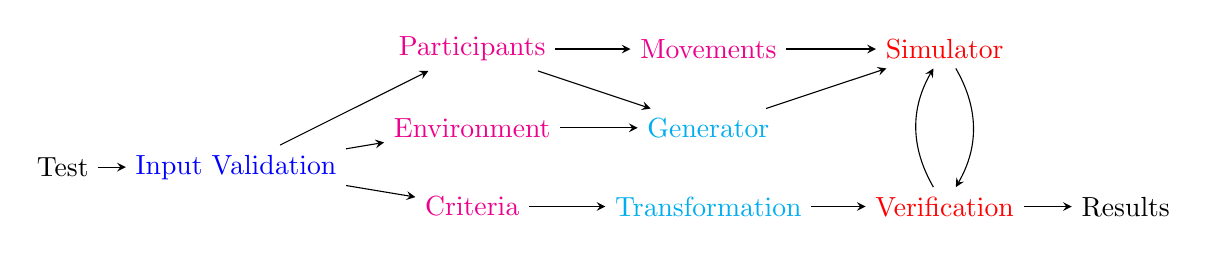
\begin{tikzpicture}[%
            ->,
            >=stealth
        ]
        \node at (-3.2,0) (Tester) {Test};
        \node at (-1,0) (Validation) {\textcolor{blue}{Input Validation}};
        \node at (2,0.5) (Environment) {\textcolor{magenta}{Environment}};
        \node at (2,1.5) (Participants) {\textcolor{magenta}{Participants}};
        \node at (5,1.5) (Movements) {\textcolor{magenta}{Movements}};
        \node at (2,-0.5) (Criteria) {\textcolor{magenta}{Criteria}};
        \node at (5,-0.5) (Transform) {\textcolor{cyan}{Transformation}};
        \node at (5,0.5) (Generation) {\textcolor{cyan}{Generator}};
        \node at (8,1.5) (Simulation) {\textcolor{red}{Simulator}};
        \node at (8,-0.5) (Verification) {\textcolor{red}{Verification}};
        \node at (10.3,-0.5) (Results) {Results};
        \path
            (Tester) edge (Validation)
            (Validation) edge (Environment)
            (Environment) edge (Generation)
            (Generation) edge (Simulation)
            (Validation) edge (Participants)
            (Participants) edge (Movements)
            (Movements) edge (Simulation)
            (Participants) edge (Generation)
            (Validation) edge (Criteria)
            (Criteria) edge (Transform)
            (Transform) edge (Verification)
            (Verification) edge[bend left] (Simulation)
            (Simulation) edge[bend left] (Verification)
            (Verification) edge (Results);
    \end{tikzpicture}
\end{figure}
The input validation checks whether the test case is broken or malformed based on the appropriate \glspl{xsd}.
If the test case is valid the environment, the criteria and the participants are extracted.
The information about lanes and obstacles in the environment is passed to the generator creating representations compatible with the simulator.
The generator also creates a participant for each specified initial state and adds it to the simulation.
The movements of the participants are passed to the simulator that applies these sequentially after the simulation started.
\draft{TODO Mention triggers in the simulation?}
The defined criteria are transformed to a Kleene and Priest logics expression that can be evaluated by the verification process during the simulation.
Then the simulator starts the test and the interaction with the verification process.
This interaction is described more detailed in \autoref{sec:runtimeVerification}.
As soon as the verification process determined whether the test succeeded or failed it stops the simulation and returns the test results.

{\bfseries Proposed tools:} I will use \beamng{}~\cite{beamNG} as simulator since it provides very accurate physics and therefore accurate test results plus it comes with the Python interface BeamNGpy~\cite{beamngpy} that allows to control simulator instances, to create scenarios dynamically and to retrieve sensor data from participants.
Furthermore \beamng{} comes with the ability of pixel perfect annotation which some \glspl{adas} need.
The input validation, the extraction, the generator, the transformation and the verification will be done in Python since the interface of \beamng{} is written in Python too and thus the interaction is easy and the interoperability is high.

\subsection{Runtime Verification}\label{sec:runtimeVerification}
The runtime verification implements the interaction between a simulator and the verification of test criteria deciding whether a test succeeded or failed.
It follows the synchronous simulation strategy to make sure that the point in time where \glspl{ai} have to control \glspl{av} is not influenced by network latency or the current load of the underlying hardware.
\begin{figure}
    \centering
    \caption{%
        Runtime verification --- Depicts the main execution loop of the interaction between a simulator and a verification process (See \autoref{fig:testCycle}).
    }\label{fig:runtimeVerification}
    \medskip
    \smartdiagram[flow diagram:horizontal]{%
        Verify criteria, Request \glspl{ai}, Control, Start Resume, Pause
    }
\end{figure}
The main execution loop realizing synchronous simulation is shown in \autoref{fig:runtimeVerification}.\\
The runtime verification starts with evaluating the preconditions, success and fail criteria and determines the verification result based on the state machine shown in \autoref{fig:verificationDecision}.
\begin{figure}
    \centering
    \caption{%
        Verification state machine --- Shows the state machine for determining the current state of the test case execution based on the evaluation of preconditions, success and fail criteria.
        Underlined nodes are final states and arrows describe the transition from node to node depending on whether a criterion evaluated to \textcolor{green}{true}, \textcolor{red}{false} or \textcolor{blue}{unknown}.
    }\label{fig:verificationDecision}
    \medskip
    \begin{tikzpicture}[%
        ->,
        >=stealth
    ]
    \node (start) {};
    \node[right=of start] (preconds) {Preconditions};
    \node[below=of preconds] (skipped) {\underline{skipped}};
    \node[right=of preconds] (fail) {Fail criteria};
    \node[below=of fail] (tcFail) {\underline{failed}};
    \node[right=of fail] (success) {Success criteria};
    \node[below=of success] (tcSuccess) {\underline{succeeded}};
    \node[right=of success] (undetermined) {\underline{undetermined}};

    \path (start) edge (preconds);
    \draw[red] (preconds) edge (skipped);
    \draw[green] (preconds) edge[bend left] (fail);
    \draw[blue] (preconds) edge[bend right] (fail);
    \draw[green] (fail) edge (tcFail);
    \draw[red] (fail) edge[bend left] (success);
    \draw[blue] (fail) edge[bend right] (success);
    \draw[green] (success) edge (tcSuccess);
    \draw[red] (success) edge[bend left] (undetermined);
    \draw[blue] (success) edge[bend right] (undetermined);
    \end{tikzpicture}
\end{figure}
If the verification ends in one of the final states \code{SKIPPED}, \code{FAILED}, \code{SUCCEEDED} or \code{TIMEOUT} the simulation stops and returns the final state.
In this case all \glspl{ai} registered at the simulation are told to stop too.
Otherwise the verification yields \code{UNKNOWN} and the runtime verification continues with the main execution loop.
If the runtime verification continues it searches for all \glspl{av} that are according to their movement currently controlled by an \gls{ai} and that have to be requested according to the request frequency and the current time of the simulation (in ticks).
Using the connections \glspl{ai} opened at \drivebuild{} the runtime verification requests them for commands controlling the simulator or an \gls{av} associated with them.
\autoref{fig:aiSimProtocol} depicts the four-way protocol which is used for the communication.
The first message registers an \gls{ai} at a simulation waiting for being requested.
Its response response contains the current state of the simulation which is either \code{RUNNING}, \code{FINISHED}, \code{CANCELED}, \code{TIMEOUT} or \code{UNKNOWN}.
This allows an \gls{ai} to recognize whether the simulation still runs or stopped.
If the simulation still runs the \gls{ai} requests properties of the current state of the associated \gls{av} and its available sensor data needed for the calculations of the \gls{ai}.
%\draft{FIXME List available data?}
The response to these requests contains the appropriate data in a serialized form.
After receiving the data the \gls{ai} starts to calculate control commands for either controlling the simulator (\eg{} interrupt it) or for controlling the associated \gls{av} with values for acceleration, brake intensity and steering angle.
The opportunity to send commands controlling the simulator instead of the \gls{av} allows an \gls{ai} to evaluate additional constraints that extend the specified test criteria and thus eventually force a test to succeed, fail or to be skipped.\\
The control step applies the commands the runtime verification received appropriately to the simulator or the correct \gls{av}.
If the simulator does not get a command to stop it starts the test case execution respectively resumes it if it was paused previously.
The simulator calculates the next tick, pauses the simulation and the runtime verification starts over again.

{\bfseries Proposed tools:} The exchange of messages and data will be based on \protobuf~\cite{protobuf} since it allows to define messages in a programming language neutral way and is able to cross compile classes for serializing messages in many languages including Python.
\begin{figure}
    \centering
    \caption{Communication between a simulation controller and an \glstext{ai} --- Visualizes the messages sent for exchanging data between a simulator and an \glstext{ai}.}\label{fig:aiSimProtocol}
    \medskip
    \includegraphics[page=1]{pictures/aiSimCommunication.pdf}
\end{figure}

\subsection{Cluster Architecture}
The architecture uses a client server model and is depicted in \autoref{fig:systemArch}.
\autoref{fig:distributeNodes} shows the distribution of the system over the cluster.
\begin{figure}
    \centering
    \caption{%
        Cluster architecture --- Visualizes all components of the cluster and the data flow between them.
        The components in the blue area belong to the client side and the components in the green area belong to the cluster.
        The orange area contains cluster components that build the micro service based accessible interface.
        \draft{FIXME Still StatsManager?}
    }\label{fig:systemArch}
    \medskip
    \begin{tikzpicture}[%
        ->,
        >=stealth
    ]
    \tikzset{%
        node distance=2
    }
    \node (tester) {Tester};
    \node[below=of tester] (tcmanager) {TCManager};
    \node[right=of tester] (ai) {\glstext{ai}};
    \node[below=of ai] (communicator) {Communicator};
    \node[below=4 of tcmanager] (simcontroller) {SimController};
    \node[left=of simcontroller] (transformer) {Transformer};
    \node[left=of transformer] (generator) {Generator};
    \node[above=of transformer] (dbms) {\glstext{dbms}};
    \node[left=4 of tcmanager] (stats) {StatsManager};
    \node[above=of stats] (researcher) {Researcher};
    \node[below=of transformer] (kptransformer) {KPTransformer};
    \node[below=of simcontroller] (verificator) {Verificator 1\ldots N};
    \node[right=0.5 of verificator] (simulatorA) {Simulator 1\ldots N};

    \node[zlayer=back,fill=blue!20,fit={(researcher)}] (clientLeft) {};
    \node[zlayer=back,fill=blue!20,fit={(tester)(ai)}] (clientRight) {};
    \node[zlayer=back,fill=green!20,fit={(simulatorA)(communicator)(dbms)(stats)(kptransformer)(tcmanager)(verificator)(generator)}] (server) {};
    \node[zlayer=back,fill=orange!20,fit={(tcmanager)(communicator)}] (microserviceA) {};
    \node[zlayer=back,fill=orange!20,fit={(stats)}] (microserviceB) {};

    \path
        (tester) edge[bend right] node[rotate=90,above]{Test case} (tcmanager)
        (dbms) edge (stats)
        (stats) edge (researcher)
        (researcher) edge (stats)
        (simcontroller) edge (dbms)
        (simcontroller) edge (transformer)
        (transformer) edge (simcontroller)
        (tcmanager) edge[bend right] node[rotate=-90,above]{Result} (tester)
        (transformer) edge node[rotate=90,above]{Test criteria} (kptransformer)
        (kptransformer) edge (transformer)
        (transformer) edge node[above]{lanes, \glspl{av}, obstacles} (generator)
        (generator) edge (transformer)
        (tcmanager) edge[bend right] node[rotate=90,above]{Scenario} (simcontroller)
        (simcontroller) edge[bend right] node[rotate=-90,above]{Result, Status} (tcmanager)
        (simcontroller) edge node[rotate=90,above]{runtime} (verificator)
        (verificator) edge node[rotate=90,below]{verification} (simcontroller)
        (simcontroller.south east) edge (simulatorA)
        (simulatorA) edge (simcontroller.south east)
        (simcontroller.north east) edge (communicator)
        (communicator) edge (simcontroller.north east)
        (communicator) edge (ai)
        (ai) edge (communicator);
    \end{tikzpicture}
\end{figure}
The functionality of the cluster is provided through micro services~\cite{microServices}.
The use of micro services allows hiding and strictly separating functionality plus it allows more granularity than other architectures like \gls{soa}.
The cluster offers multiple services.\\
The TCManager service implements methods for accepting test cases of a tester, checking their validity, passing them to the transformer, triggering the execution of test cases, monitoring the execution, returning test case results to the tester and to store results in a \gls{dbms}.
The Transformer (transformation step in \autoref{fig:testCycle}) accepts validated test cases, extracts information about the environment and the participants, generates representations which are compatible with the simulator, extracts the test criteria and transforms them to an expression that can be evaluated during the simulation.
The SimController manages all simulator instances as well as their verification instances and implements the runtime verification described in \autoref{sec:runtimeVerification}.
It also provides methods for requesting the current status of test executions which the TCManager requires for monitoring.
The Communicator service handles the exchange of messages between a simulation controlled by the SimController and an \gls{ai} controlling an \gls{av} of a scenario and thus uses the protocol visualized in \autoref{fig:aiSimProtocol}.
\draft{FIXME Still StatsManager?}
The StatsManager service grants access to the data stored by the TCManager in the \gls{dbms} enabling researchers to investigate and analyze collected data about test case executions.\par

\begin{figure}
    \centering
    \caption{%
        Distribution over the cluster --- Visualizes how the components shown in \autoref{fig:systemArch} are distributed over multiple nodes.
        The blue node represents a client node, the orange node represents a \gls{vm} providing the micro service layer and the green nodes represent the cluster nodes as well as the \gls{dbms}.
    }\label{fig:distributeNodes}
    \medskip
    \begin{tikzpicture}[%
            ->,
            >=stealth
        ]
        \node (client) {\includegraphics[width=.125\linewidth]{pictures/computer_client.png}};
        \node[right=1.5 of client] (microService) {\includegraphics[width=.125\linewidth]{pictures/virtualMachine_microService.png}};
        \node[right=1.5 of microService] (windows2) {\includegraphics[width=.0625\linewidth]{pictures/virtualMachine_windows.png}};
        \node[above=0.5 of windows2] (windows1) {\includegraphics[width=.0625\linewidth]{pictures/virtualMachine_windows.png}};
        \node[below=0.25 of windows2] (dots) {\vdots};
        \node[below=0.25 of dots] (windows3) {\includegraphics[width=.0625\linewidth]{pictures/virtualMachine_windows.png}};
        \node[right=1.5 of windows2] (dbms) {\includegraphics[width=.0625\linewidth]{pictures/dbms.png}};

        \node[below=0.2 of windows3] (windowsTitle) {Cluster};
        \node[right=1.3 of windowsTitle] (dbmsTitle) {\glstext{dbms}};
        \node[left=1.2 of windowsTitle] (microServiceTitle) {MicroServices};
        \node[left=1.8 of microServiceTitle] (clientTitle) {Client};

        \draw
            (client) edge (microService)
            (microService) edge (client)
            (microService) edge (windows1)
            (windows1) edge (microService)
            (microService) edge (windows2)
            (windows2) edge (microService)
            (microService) edge (windows3)
            (windows3) edge (microService)
            (dbms) edge (windows1)
            (windows1) edge (dbms)
            (dbms) edge (windows2)
            (windows2) edge (dbms)
            (dbms) edge (windows3)
            (windows3) edge (dbms)
            (microService) edge[bend left=70] (dbms) % FIXME These two edges needed?
            (dbms) edge[bend right=70] (microService);
    \end{tikzpicture}
\end{figure}

{\bfseries Proposed tools:} I will use \postgresql{} since many languages provide good support, it is well known and thus bullet proven.
The micro services will be based on Flask~\cite{flask} since it is written in Python providing high compatibility with other components and it allows to use \gls{html} templates.\draft{FIXME Templates relevant?}
